%
% Copyright (c) 2011-2013, fortiss GmbH.
% Licensed under the Apache License, Version 2.0.
% 
% Use, modification and distribution are subject to the terms specified
% in the accompanying license file LICENSE.txt located at the root directory
% of this software distribution. A copy is available at
% http://chromosome.fortiss.org/.
%
% This file is part of CHROMOSOME.
%
% $Id: xme_overview.tex 7852 2014-03-14 16:32:01Z geisinger $
%

\section{\xme in a Nutshell (30 minutes)}
\label{sec:architecture}

\xme (often abbreviated by ``XME'') is a domain-independent, data-centric\footnote{%
For details, please refer to \url{http://www.omg.org/news/whitepapers/Intro_To_DDS.pdf}}
middleware for cyber-physical systems.
%
From the point of view of an application component,
\xme abstracts from basic functionality that is traditionally found in operating systems and middlewares,
like scheduling and communication.
Apart from that, it offers model-driven design tools with code generation capabilities
that allow a user to design the distributed system in an abstract way.
%
This section will give the reader a very high level overview of the most important \xme features.
For in-depth information and concrete specifications, the reader is kindly referred to the commented source code of \xme.

\subsection{Goals of \xme}
\xme is designed to match the requirements of future cyber-physical systems.
As a research prototype, the main intention is to serve as a basis
for discussion how future middleware/operating system architectures may look like.
The development is done in a demand-driven way.
Depending on the requirements of projects where \xme is applied, new features in \xme will be introduced.

Our point of view is that
future middleware will not operate on a specific class of devices, but will run on very heterogeneous platforms.
The exaggerated goal statement could be to ``develop a middleware serving a range from 8-bit controllers to cloud servers''.\footnote{%
	This is a very striking motto.
	The functionality offered by the middleware will of course vary depending on the resource constraints of the target platform.
}
%
Hence, scalability and modularity of the middleware is of highest importance. It must be easy to remove or add components from/to 
the middleware. Similar to micro-kernel operating systems, the core of \xme must be very small and only contain the absolutely necessary
features. Since the boundaries of operating systems, middleware, and applications are vanishing, one unique mechanism must be supported to
add components on all these levels.

%\paragraph{Concept 1: Data-Centric Design}
\paragraph{Data-Centric Design}
A very successful concept to achieve scalability is message-orientation as for example demonstrated by the QNX\footnote{\url{http://www.qnx.com/}} neutrino micro-kernel.
However, one major drawback of this concept is the necessity of requiring knowledge of both the sender and the receiver.
In the context of systems-of-systems where the communication partners are not known at design time, message orientation cannot be applied.
Therefore, \xme is based on the very powerful concept of data-centric design. Components specify which data they consume
and produce and depending on this information, the middleware calculates the communication routes.

It is important to note that in contrast to prominent other middleware systems relying on data-centric design,
\xme does not broadcast the data, instead it calculates specific routes based on the requirements.
This allows for a very efficient implementation. Furthermore, the routes are calculated only when components are added or removed. Based
on the experience in embedded systems, we assume that reconfiguration takes place less often than the transmission of data items.
Similar to concepts from multimedia protocols,
our initial assumption is that data transmission has to happen within real-time,
while reconfiguration is not time-critical or has only soft real-time requirements.

Data is grouped by so-called \emph{topics}. A topic is a data type with a certain structure.
Examples for topics are \emph{temperature}, \emph{rotation speed} or \emph{GPS position}. Topics are defined for a specific domain.
This enables the exchange of data between different applications.
%To allow cross-domain communication, we plan to define translation matrixes between the topics of different domains.
%
Topics are organized in so-called \emph{topic dictionaries}.
Each dictionary contains topic definitions for a specific domain and/or application.

%\paragraph{Concept 2: Refinement of Topics with Attributes}
\paragraph{Refinement of Topics with Attributes (partially implemented)}
Exchange of data can only be automated if the requirements on data are specified explicitly.
This includes information about the quality of data such as \emph{age}, \emph{accuracy}, \emph{confidence} and \emph{safety level}.
In the respective topic dictionary, each topic can be annotated with so-called \emph{attributes}.\footnote{Called \emph{meta-data} in previous versions of \xme.}
An attribute consists of a \emph{key} (its name) and its \emph{value}.
Depending on the type of attribute, the concrete value may be constant, known at configuration time or dynamically calculated during runtime.
%\TODO{[REWORK]
%\begin{itemize}
	%\item \textbf{Static meta-data:}
		%Application components have fixed requirements and guarantees.
		%Meta-data are used to calculate the appropriate communication routes at configuration time.
		%For example, imagine a temperature sensor network for building automation.
		%Depending on its size, multiple sensors may be present in a room.
		%Each sensor would specify its \emph{location} as meta-data.
		%A climate control component that controls the air conditioning system for a specific room would specify, using meta-data,
		%that it only wants to receive temperature data from sensors that match the respective room.
	%
	%\item \textbf{Dynamic meta-data:}
		%Application components producing data may specify meta-data such as the quality of the transmitted values dynamically during runtime.
		%Consuming components may have dynamic meta-data acceptance filters and may use meta-data also for their calculations.
		%For example, imagine that one of the rooms in the auotmated building from the previous example is a server room.
		%In this case, a high reliability is required.
		%Using meta-data about the confidence of each sensor,
		%the climate control may dynamically calculate the confidence in its own set value for the air conditioning system.
		%The association of data from the respective room could still use static meta-data.
%\end{itemize}
%}
%
Using attributes, application components describe their requirements respectively guarantees on data.
This information can be used to select appropriate communication streams while still retaining independence between sender and receiver.

%\paragraph{Concept 3: Data Access}
%Components can access data in two different ways. As standard operation, \xme provides a publish-subscribe mechanism. Each component states
%which data is required and which data is produced. The middleware ensures the routing of the specific data. If data is only required 
%seldomly in comparison to the data production rate, a request-response mechanism is offered to the application developer.

%\paragraph{Concept 4: Timing (not yet implemented)}
\paragraph{Model of Execution (partially implemented)}
Correct timing is a major concern for cyber-physical systems.
\xme abstracts the concrete implementation, but currently offers mechanisms to specify schedules for time-triggered execution.
In future versions, end-to-end-timing and jitter requirements for data paths will also be supported.

The reason to abstract the concrete implementation/concrete configuration
in \xme is on the one hand to reduce the development effort by automatically deriving a concrete configuration satisfying the timing
requirements (if a configuration exists) and on the other hand to support plug~\&~play capability. The state of the art in embedded system
design requires the developer to configure the application in a correct way. Several configurations might be valid, but typically only one
configuration is specified. It is not possible for the run-time system to change the configuration, as the real requirements are not present
any more and the system can not calculate alternative configurations. By explicitly stating the requirements and leaving configuration issues
to the run-time system, this problem can be avoided.
The system can support new components by calculating a new configuration that satisfies both
the requirements of already running applications and the newly installed applications.

It is important to note that \xme can of course only offer guarantees that are enabled by the underlying platform.
In case \xme runs on a Linux or Windows system without real-time kernel/extensions,
\xme will not be able to satisfy jitter requirements in the range of microseconds.
Nevertheless, certain implementations on top of such systems may offer very good guarantees.
The major concept here is to use algorithms that offer determinism sacrificing average-case performance.
Examples are the implementation of a time-triggered communication scheme on top of Ethernet.
This implementation guarantees collision free communication, but comes with a lower bandwidth and flexibility.

%\paragraph{Concept 5: Resource-Awareness (not yet implemented)}
%\xme is designed to be able to handle all resources of the platform.
%The major idea is that components/applications can state their worst-case resource requirements
%on memory, computation time, bandwidth, etc.
%\xme will then ensure that enough resources are available to allow the execution of this component/application.
%
%\paragraph{Concept 6: Other extra-functional properties -- Fault-tolerance, QoS, Security (not yet implemented)}
%\xme is designed in a way such that components which guarantee other extra-functional properties can be easily extended.
%Examples on extra-functional properties that are currently being integrated in \xme are fault-tolerance, QoS, and security.
%
%\paragraph{Concept 7: Support for States (not yet implemented)}
%A very important topic to ensure resource efficiency is state awareness.
%We are currently thinking about possibilities to support states
%(each one with a set of active applications) in \xme.
%The support of (sub-)system wide states would simplify the development of applications,
%but also other aspects such as fault-tolerance.

\paragraph{Plug \& Play}

One of \xme's major goals is to allow dynamic reconfiguration of a distributed application at runtime.
In order to combine this concept with real-time capabilities and determinism, we distinguish between the so-called \emph{plug phase} and the \emph{play phase}.
The plug phase, which is entered upon startup and can on demand be triggered during runtime,
is used to analyze the requirements of all components and to develop a plan for configuring the runtime system in order to meet the dependencies.
The plug phase is not real-time capable, i.e., its exact duration is not guaranteed.
During the plug phase, component requirements are checked, binaries are copied, data paths are calculated and the configurations for every element in the system are prepared and deployed.
For this purpose, plug \& play related components on all nodes in the network cooperate.

When the configuration is finished, the system transitions to the play phase.
The play phase is deterministic with respect to the requirements stated by the components, such as the worst-case execution time.

Subsequent plug \& play events may be triggered in the play phase,
for example node plugout (i.e., the removal of nodes from the XME ecosystem)
or removal of individual components.

\paragraph{Health Monitoring (partially implemented)}

Although the system is deterministic during the play phase, a runtime health monitoring is required,
because an application component might violate its asserted requirements.
For example, an application component might violate its worst-case execution time or try to access a resource where it has no access to.
Similarly, a network communication problem might occur.
In such cases, the system is supposed to fall back into a safe mode in which the basic functionality of the application is retained.
This allows for safe ``shutdown''.

\subsection{Glossary}
\label{sec:architecture:glossary}

This glossary explains the most important terms in \xme in alphabetical order.

\paragraph{Component}
A component is a modular software unit that has input and output interfaces, so-called \emph{ports}.
A component consist of at least one \emph{function}.

\paragraph{Component Wrapper}
A component wrapper is the interface between a component and the \emph{Data Handler} core component.
For every input port of the respective component, it offers a respective reading function.
For every output port of the respective component, it offers a respective writing function.
The reading and writing functions are called by the component's functions.
The component wrapper enforces the isolation between \xme core components and (untrusted) functions with respect to data passing.

\paragraph{Ecosystem}
A collection of \xme nodes that communicate with each other.
Nodes can be added to and removed from an \xme ecosystem via plug \& play.

\paragraph{Function}
A function is a primitive algorithm that is associated with a \emph{component}.
It may read a subset of its \emph{component}'s input \emph{ports} and may write a subset of its \emph{component}'s output ports.
Functions are annotated with their worst-case execution time.

\paragraph{Function Wrapper}
The function wrapper is the interface between the \emph{Execution Manager} component and a function.
Whenever the \emph{Execution Manager} runs a function, it does not directly call the function,
but instead it unblocks the thread that executes the respective function wrapper.
The function wrapper then ensures that all data that the respective function needs are readily available and then calls the function.
When the function returns, the function wrapper signals the \emph{Execution Manager} accordingly.
The function wrapper enforces the isolation between \xme core components and (untrusted) functions with respect to execution.

\paragraph{Node}
In terms of \xme, a node is an instance of the \xme runtime system that implements a certain part of a (possibly distributed) application.

\paragraph{Node Identifier}
A node identifier is a number uniquely identifying a \emph{node} in a \xme network.
Node identifiers are maintained by the \emph{Login Manager}.

\paragraph{Play Phase}
Time where the distributed system is running in order to achieve the intended task.
Opposite of \emph{plug phase}.

\paragraph{Plug Phase}
Time where the distributed system is being configured or reconfigured automatically, depending on specified requirements.
Plug phase is entered on system startup or on request by the user or \emph{Plug \& Play Manager}.
Opposite of \emph{play phase}.

\paragraph{Port}
A port is an input or output interface of a component.
Ports are associated with a specific \emph{topic} that defines the type of data expected respectively emitted by the port.
Ports may be implemented by a single memory cell, a queue, or a ring buffer, for example.
A port specifies whether it is persistent, that is whether the last received value contained in a port will be kept around for further read operations or not.

\paragraph{Topic}
A topic is a type of data transmitted between \emph{ports} of \emph{components}.

\paragraph{Waypoint}
A waypoint is a lightweight component that applies a certain transformation to data.
For example, marshaling and demarshaling are two waypoints.
Likewise, sending and receiving of data according to a specific protocol are represented by two waypoints.\footnote{%
	In previous versions of \xme, the now obsolete \emph{Interface Manager} was responsible for transferring data over the network.
}
Waypoints have a configuration interface which is used to ``program'' their tasks during \emph{plug phase}.
During \emph{play phase}, waypoints deterministically achieve their task according to their configuration.

\begin{figure}[htb]
	\centering
	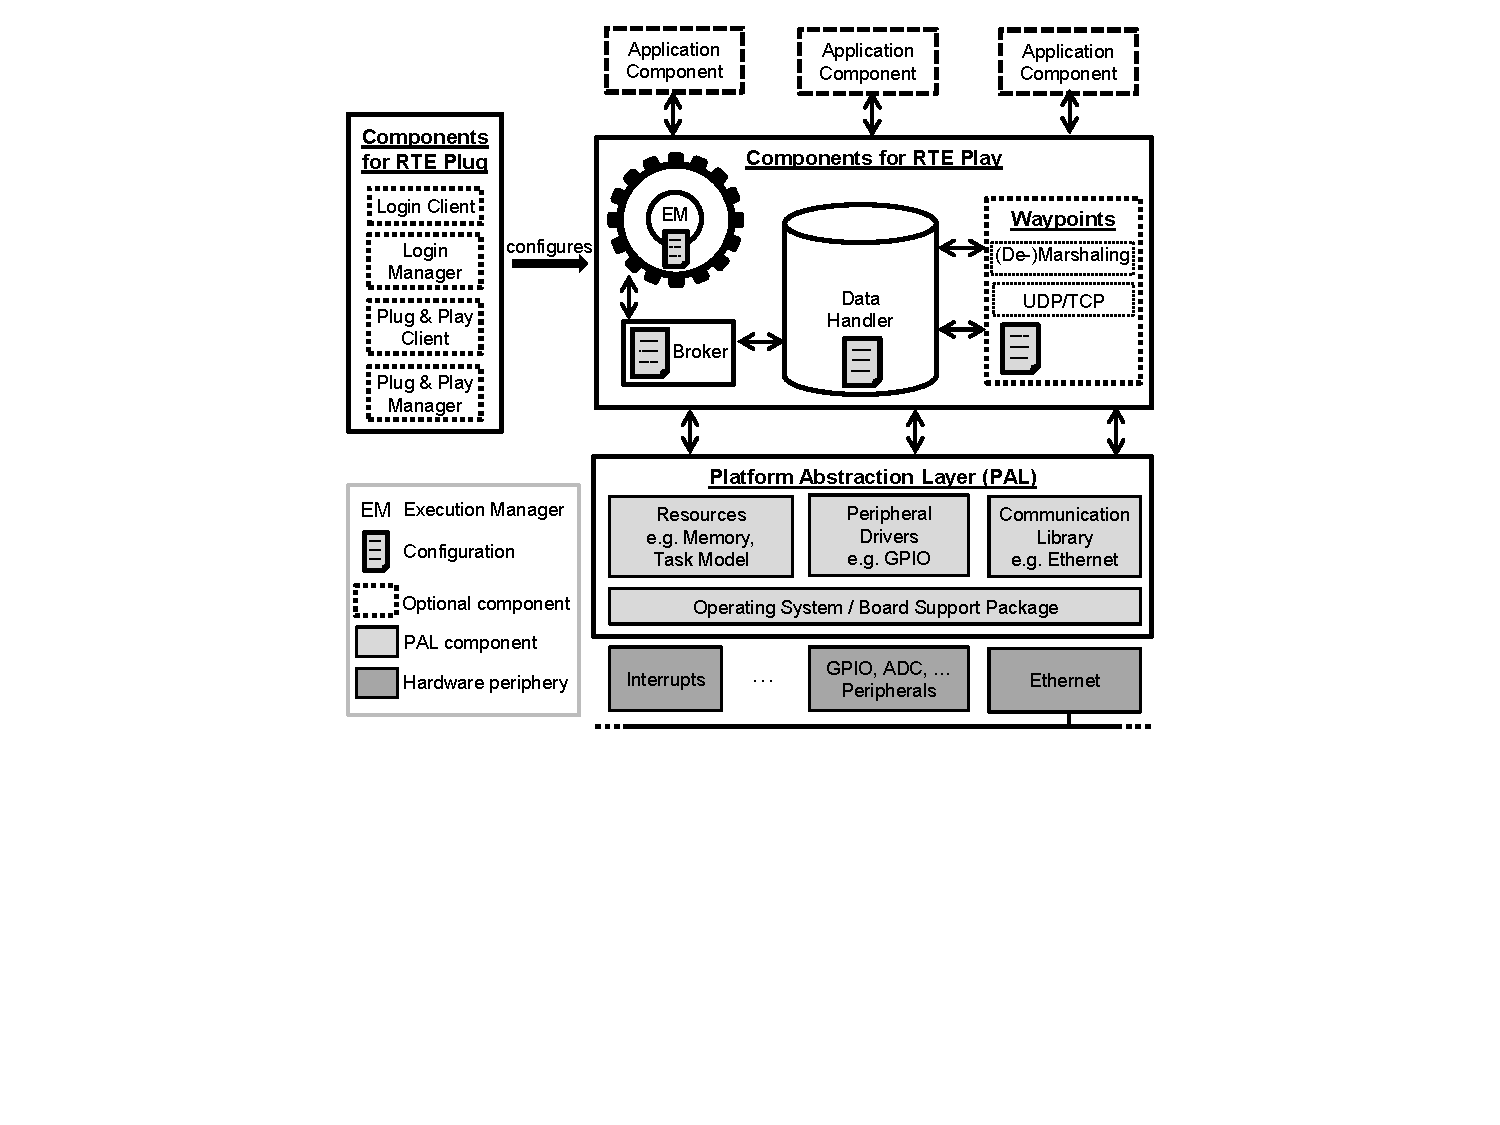
\includegraphics[width=0.8\textwidth,trim=166 190 166 5]{figures/architecture.pdf}
	\caption{\xme architecture overview.}
	\label{fig:architecture}
\end{figure}



\subsection{\xme Components}

\label{sec:core_components}
\xme is designed in a modular fashion. Its component-oriented architecture is depicted in Figure~\ref{fig:architecture}.
A (distributed) \emph{application} consists of a set of (software) \emph{components} that interact with each other by exchanging data.
Each component is placed on a specific \emph{node} in the network.
On operating system based platforms like Linux or Windows,
the software of a node is typically represented by a console application.
On embedded systems, the software of a node corresponds to the firmware.
A component may contain a number of \emph{functions} that exchange data via the \emph{ports} of their parent component.
A component's \emph{input port} may receive data from other components and forward it to one of its functions for processing.
Functions may generate data for publication on their parent component's \emph{output ports}.

The following sections provide brief descriptions of the most important components of \xme.
See Figure~\ref{fig:architecture} for a graphical illustration.



\subsubsection{Mandatory Components for RTE Play}

``RTE play'' refers to the normal execution of a \xme node.

\paragraph{Broker}
The Broker ``knows'' which function depends on which data in the input ports of their parent components.
As such, it knows when a function has enough data to be executed.
When data is available on an output \emph{port} of a \emph{component}, the Broker copies them to the dependent input \emph{ports} by triggering a transfer function in the \emph{Data Handler}.
Hence, the Broker offers an interface where the \emph{Execution Manager} can query whether a function is currently ready for execution.\footnote{%
	In previous versions of \xme, the Broker was responsible for delivering data to components.
	In this version of \xme, the actual transfer is achieved by the \emph{Data Handler}.
}

\paragraph{Execution Manager}
The Execution Manager is responsible for executing functions that are ready for execution.
Depending on the model of execution (currently, only time triggered execution is supported),
the Execution Manager has a set of schedules (time triggered) or priorities (event triggered), or both (hybrid).

In the time triggered case, the Execution Manager executes checks for every component
whether it is ready for execution in a round-robin fashion.
For this purpose, it asks the \emph{Broker} whether the data dependencies of the respective function are satisfied.
Under all functions that are ready for execution, the Execution Manager chooses one to execute.
While a function is executed, it reads data from the ports of the respective component (by calling respective functions in the \emph{Data Handler}).
This may lead to the function not being executable any more in the next cycle.

\paragraph{Data Handler}

The Data Handler offers a central storage for all data exchanged via data centric communication ports of components on a node.
The \emph{component wrappers} interact with the Data Handler by reading and writing data and attributes.



\subsubsection{Optional Components for RTE Plug}

``RTE plug'' refers to reconfigurability aspects of \xme.

\paragraph{Logical Route Manager}
The Logical Route Manager (not shown in Figure~\ref{fig:architecture})
receives a list of all publications and subscriptions from the \emph{Plug \& Play Manager}
when the system configuration is to be updated (\emph{plug phase}).
Based on this information, the Logical Route Manager calculates logical routes,
i.e., it finds sources and sinks with matching topics and attributes.
The set of logical routes is forwarded to the \emph{Network Configuration Calculator}.

\paragraph{Network Configuration Calculator}
The Network Configuration Calculator (not shown in Figure~\ref{fig:architecture}) takes the logical routes calculated by the \emph{Logical Route Manager}
and enhances them with communication protocol specific transformation steps that are applied to the data
in between the sender (publication) and the receiver (subscription).
We call such transformations \emph{waypoints} on the data path.
Furthermore, the Network Configuration Calculator calculates where in the network the individual waypoints are to be placed.
The result is a set of physical routes and deployment information that is sent back to the \emph{Plug \& Play Manager}.

\paragraph{Plug \& Play Manager}
The Plug \& Play Manager is responsible for handling requests for dynamic changes to the running system.
It is also responsible for the startup procedure.
The Plug \& Play Manager is either triggered by a system reset, by the user, or by the login or logout of a node in the network.
It calculates the set of changes that will be applied to the system and triggers other components accordingly,
such as the \emph{Logical Route Manager}, the \emph{Network Configuration Calculator}, or the \emph{Plug \& Play Clients} on remote nodes.
Only one Plug \& Play Manager should exist in a network.

\paragraph{Plug \& Play Client}
The Plug \& Play Client (not shown in Figure~\ref{fig:architecture}) receives commands from the \emph{Plug \& Play Manager} that is present on a specific node in the network.
It interprets those commands and adapts the configuration of local components accordingly, such as the \emph{Broker}, the \emph{Data Handler}, and the \emph{Execution Manager}.

\paragraph{Login Client}
The Login Client (not shown in Figure~\ref{fig:architecture}) is responsible for connecting a node
to other nodes in the network and obtaining a so-called \emph{node identifier}.
The node identifier is a unique address of the node within a network.
The Node Manager periodically tries to obtain such a node identifier from the \emph{Login Manager},
which is present on one specific node in the network.
%
This component is optional, because in statically configured networks, no login or logout might be necessary or supported.

\paragraph{Login Manager}
The Login Manager receives login requests from the \emph{Login Client}s of all other nodes and handles them by assigning respective \emph{node identifiers}.
Only one Login Manager should exist in a network.

\paragraph{Node Manager}
A node can have an arbitrary amount of software components that implement the application.
The Node Manager (not shown in Figure~\ref{fig:architecture}) provides management mechanisms for managing existing components and instantiating new components.



\subsubsection{Primitive Components}

Primitive Components directly access the \emph{Hardware Abstraction Layer} using function calls
and offer data obtained from the hardware in a data centric way or forward data to the respective actuators.
They are typically the source of physical data obtained from the environment and
the sink for control data to the environment.



\subsubsection{Platform/Hardware Abstraction Layer}

The Platform/Hardware Abstraction Layer, often abbreviated by PAL or HAL,
provides a platform independent application programming interface (API).
\xme \emph{components} are usually implemented against that API and are hence platform independent.
The HAL implements hardware-specific functionality such as drivers for microcontroller periphery
like general purpose I/O (GPIO) or analog to digital conversion (ADC),
but it also provides a lot of software functions similar to an operating system.
See the content of the directory \verb|<XME_ROOT>/xme/hal/include|\footnote{%
	\texttt{<XME\_ROOT>} specifies the root of the \xme source package.
	See Chapter~\ref{sec:example_sensorMonitor} for details.
}
for an overview of the supported functionality.
Each header file in this directory corresponds to a HAL module
and contains documentation about the provided functionality.

\subsubsection{Application Components}

The actual (distributed) application running in the network is implemented by specific Application Components.
They typically operate only on data obtained via data centric communication.
In particular, no direct access to the Hardware Abstraction Layer with effects in the environment should be made,
instead Application Components should use \emph{Primitive Components}.
This design concept leads to modular, reusable components.



%\subsubsection{IP Login Client Proxy and IP Login Manager Proxy}
%
%These components are required for new nodes to initially contact the Login Manager.
%A node that does not have a Login Manager will usually have a \emph{Login Manager Proxy} component for each of its physical network interfaces.
%These components are named according to their associated interface types,
%for example \emph{IP Login Manager Proxy} for an Ethernet interface with IP communication stack.
%Whenever the Node Manager, which is responsible for periodic login requests, issues a login request,
%the Login Manager Proxy takes care of broadcasting it over its associated communication interface.
%
%Nodes that have a Login Manager component usually also have a \emph{Login Client Proxy} for each of their interfaces.
%The Login Client Proxy will receive the login requests issued by the Login Manager Proxy on the respective medium
%and forward them locally to the Login Manager.
%The login response is forwarded in a similar manner.
%%
%This concept makes it possible to separate the login and address assignment logic from specific interface types and communication protocols
%and enables a fine-grained assignment of functionality to each communication interface.



%\subsection{Component Definition and Lifecycle}
%\label{sec:component_definition}
%
%\xme \emph{components} are assigned to one of the following categories according to their ``layer'' within the system:
%\verb|adv| (advanced), \verb|prim| (primitive), \verb|core| (runtime system), \verb|wp| (\emph{waypoint}) or \verb|hal| (hardware abstraction).
%Depending on the category, different mechanisms exist for a component to interact with its environment.
%
%A \xme component is defined by four functions to \emph{create}, \emph{activate}, \emph{deactivate} and \emph{destroy} it,
%illustrated here for a component called \verb|xme_adv_myComponent|:
%\begin{quote}
	%%\verb|xme_core_status_t|\\
	%\verb|xme_adv_myComponent_create(xme_adv_myComponent_configStruct_t*);|\\
	%%\verb|xme_core_status_t|\\
	%\verb|xme_adv_myComponent_activate(xme_adv_myComponent_configStruct_t*);|\\
	%%\verb|void|\\
	%\verb|xme_adv_myComponent_deactivate(xme_adv_myComponent_configStruct_t*);|\\
	%%\verb|void|\\
	%\verb|xme_adv_myComponent_destroy(xme_adv_myComponent_configStruct_t*);|
%\end{quote}
%%
%The distinction between creation/activation and deactivation/destruction is required in case a component needs to be migrated:
%in this case, the component is first deactivated (to obtain a consistent state), then moved and activated at the new location.
%All four functions take a pointer to a configuration structure, which represents the state of the respective component instance.
%Multiple component instances of the same component type usually have their own configuration structures.
%
%A typical task during creation of a component is registration of data demand and data production.
%Furthermore, a component may create (periodic) tasks to implement its functionality.
%These two concepts are illustrated in the following sections.
%
%\subsection{Component Instantiation}
%
%Components can be instantiated by adding them to the so-called \emph{component list}, usually defined in the main program file.
%Mandatory core components (compare Figure~\ref{fig:architecture}) are implicitly added to the list.
%An initial configuration may be provided for each component.
%Listing~\ref{lst:component_list} shows a sample component list with respective configurations.
%
%\begin{lstlisting}[numbers=left,float=htpb,label=lst:component_list,caption=Sample component list with component configurations.]
%/*****************************************************************************/
%/***   Component configurations                                            ***/
%/*****************************************************************************/
%XME_COMPONENT_CONFIG_INSTANCE(xme_core_nodeManager) = ~\label{lst:component_list.initialized_config_begin}~
%{
	%0x00000000021041A1, // deviceType
	%XME_CORE_DEVICE_GUID_RANDOM // deviceGuid
%}; ~\label{lst:component_list.initialized_config_end}~
%
%XME_COMPONENT_CONFIG_INSTANCE(xme_prim_ipLoginServerProxy, 1); ~\label{lst:component_list.uninitialized_config}~
%
%/*****************************************************************************/
%/***   Component descriptor                                                ***/
%/*****************************************************************************/
%XME_COMPONENT_LIST_BEGIN
	%XME_COMPONENT_LIST_ITEM(xme_core_nodeManager, 0) ~\label{lst:component_list.stateful_1}~
	%XME_COMPONENT_LIST_ITEM(xme_prim_ipLoginServerProxy, 0) ~\label{lst:component_list.stateful_2}~
	%XME_COMPONENT_LIST_ITEM_NO_CONFIG(xme_adv_myComponent) ~\label{lst:component_list.stateless}~
%XME_COMPONENT_LIST_END;
%\end{lstlisting}
%
%This example declares that three components (besides internal core components),
%namely \verb|xme_core_nodeManager|, \verb|xme_prim_ipLoginServerProxy| and \verb|xme_adv_myComponent|,
%will be present on this node.
%We can distinguish between the following types of components:
%\begin{enumerate}
	%\item \textbf{Components with internal state:}
		%The \verb|XME_COMPONENT_LIST_ITEM()| macro is used to declare such a component
		%(compare lines~\ref{lst:component_list.stateful_1} and~\ref{lst:component_list.stateful_2}).
		%The second parameter of the macro is the zero-based index of the respective configuration
		%(defined above the list) that is used to initialize the component.
		%
		%Some components expect some of their configuration variables to be initialized properly.
		%For example, the \emph{Node Manager} expects its \emph{device type} and \emph{device GUID}
		%members to be set up.
		%This is achived by assigning values to the respective members
		%when declaring the configuration structure with the \verb|XME_COMPONENT_CONFIG_INSTANCE| macro
		%(compare lines~\ref{lst:component_list.initialized_config_begin}--\ref{lst:component_list.initialized_config_end}).
		%Configurations for multiple components of the same type can be declared
		%by separating multiple initialization blocks with commas and using the respective index in the
		%\verb|XME_COMPONENT_LIST_ITEM()| macro.
		%
		%Other components, like the \emph{IP Login Manager Proxy}, do not require any special configuration.
		%They only need a properly defined configuration structure to store their state during runtime.
		%Again, the \verb|XME_COMPONENT_CONFIG_INSTANCE| macro is used
		%with the second parameter set to the number of configuration structures for that component type to create
		%(we could also declare multiple components of the same type), in this case one
		%(line~\ref{lst:component_list.uninitialized_config}).
	%
	%\item \textbf{Components without internal state:}
		%The \verb|XME_COMPONENT_LIST_ITEM_NO_CONFIG()| macro is used to declare such a component
		%(compare line~\ref{lst:component_list.stateless}).
		%In this case, \verb|NULL| will be passed in the \verb|config| parameters of the four functions introduced in Section~\ref{sec:component_definition}.
%\end{enumerate}
%
%The list item macro calls have to be embedded between the \verb|XME_COMPONENT_LIST_BEGIN| and \verb|XME_COMPONENT_LIST_END| macro calls.
%%
%Components declared in this list are automatically created and activated during startup
%and deactivated and destroyed during shutdown.
%
%\subsection{Sending and Receiving Data}
%
%Before sending data, a component states its intent to the runtime system.
%This is necessary to allow the appropriate communication routes to be set up
%and is usually performed from within a component's \emph{create} function.
%%
%For using data centric communication, \verb|#include| the file \verb|"xme/core/dcc.h"|.
%%
%To inform \xme that a component intends to send data under a specific \verb|topic|, call:
%\begin{quote}
	%\verb|publicationHandle =|\\
	%\verb|    xme_core_dcc_publishTopic(|\\
	%\verb|        topic, XME_CORE_MD_EMPTY_META_DATA, NULL|\\
	%\verb|    );|
%\end{quote}
%
%The actual sending of \verb|data| is performed with:
%\begin{quote}
	%\verb|xme_core_dcc_sendTopicData(|\\
	%\verb|    publicationHandle, &data, sizeof(data)|\\
	%\verb|);|
%\end{quote}
%
%A component can subscribe to a certain \verb|topic| with a given \verb|receiveTopicCallback| function by calling:
%\begin{quote}
	%\verb|subscriptionHandle =|\\
	%\verb|    xme_core_dcc_subscribeTopic(|\\
	%\verb|        topic, XME_CORE_MD_EMPTY_META_DATA, receiveTopicCallback, NULL|\\
	%\verb|    );|
%\end{quote}
%Whenever data matching the given topic is received, the given callback function is invoked.
%The last parameter of the function can be used to pass user-defined data to the callback function,
%for example a pointer to the component's configuration structure.
%%
%\verb|receiveTopicCallback| must have a signature matching \verb|xme_core_dcc_receiveTopicCallback_t|, namely:
%\begin{quote}
	%\verb|void receiveTopicCallback(xme_hal_sharedPtr_t dataHandle, void* userData);|
%\end{quote}
%\verb|dataHandle| is a reference to the memory where the received data is located.
%
%\subsection{Working with Tasks}
%
%Tasks are allocated via the resource manager,
%hence \verb|#include| \verb|"xme/core/resourceManager.h"| to use them.
%A component can create one or multiple asynchronous tasks by calling
%
%\begin{quote}
	%\verb|taskHandle = |\\
	%\verb|    xme_core_resourceManager_scheduleTask(|\\
	%\verb|        startMs, periodMs, XME_HAL_SCHED_PRIORITY_NORMAL,|\\
	%\verb|        taskCallback, NULL|\\
	%\verb|    );|
%\end{quote}
%
%This function registers the \verb|taskCallback| function to be scheduled for execution
%according to \verb|startMs| (number of milliseconds before first invocation) and
%\verb|periodMs| (interval between invocations).
%%
%The last parameter of the function can be used to pass user-defined data to the callback function,
%for example a pointer to the component's configuration structure.
%%
%\verb|taskCallback| must have a signature matching \verb|xme_hal_sched_taskCallback_t|, namely:
%\begin{quote}
	%\verb|void taskCallback(void* userData);|
%\end{quote}
%
%A task can be suspended or resumed by calling:
%
%\begin{quote}
	%\verb|xme_hal_sched_setTaskExecutionState(|\\
	%\verb|    taskHandle, <flag>|\\
	%\verb|);|
%\end{quote}
%
%\verb|<flag>| is a Boolean flag that indicates the new task execution state.
%The call will block until the new state can be enforced,
%which is not the case while the task's callback function is executed.
%%A task's callback function should return periodically
%%and the \verb|periodMs| argument in the \verb|xme_core_resourceManager_scheduleTask()| call
%%should be used to reschedule themselves at the appropriate points in time.
%%
%A task can be aborted by calling:
%
%\begin{quote}
	%\verb|xme_core_resourceManager_killTask(|\\
	%\verb|    taskHandle|\\
	%\verb|);|
%\end{quote}
%
%If this function is called from the task to kill itself, then it will mark the task for deletion and return immediately.
%If it is called from a different task, the function blocks until the task has been removed.
%Similarly to suspension and resuming, a task is not removed until its callback function has returned.
